\chapter{Badania}
\section{Wykorzystywana miara jakości klasyfikatora}
Podstawowymi miarami stosowanymi w~ocenie jakości sieci neuronowych są:
\begin{itemize}
    \item dokładność (\textit{ang.~accuracy}),
    \item średnia precyzja (\textit{ang.~average precision}).
\end{itemize}

\paragraph{Dokładność} wskazuje jaka część przykładów ze~zbioru ewaluacyjnego została sklasyfikowana poprawnie.
\begin{equation*}
    ACC = \frac{CP}{T}
\end{equation*}
gdzie $CP$ to~liczba poprawnie sklasyfikowanych przykładów, a~$T$ to~całkowita liczba przykładów.

Jeśli wśród przykładów istnieje spora nadreprezentacja przykładów jednej klasy wówczas wskaźnik ten~może być
niemiarodajny. Przykładowo: klasyfikator mający stwierdzać płeć wśród studentów Wydziału Elektroniki i~Technik
Informacyjnych Politechniki Warszawskiej mógłby wsakzywać dla~każdej osoby płeć męską, a~jego dokładność byłaby
dość wysoka. Dlatego w~takich przypadkach badając jakość sieci należy posłużyć się~również dodatkowymi miarami.

\paragraph{Precyzja} to~miara, która liczona jest dla~każdej z~klas z~osobna i~wyraża ile~przykładów sklasyfikowanych
 jako należące do~danej~klasy faktycznie należy do~tej klasy (przykładowo: jaka część obrazów sklasyfikowanych jako
 obraz z~psem faktycznie jest obrazem przedstawiającym to~zwierzę). W~ocenie jakości sieci neuronowych rozpoznających
 więcej niż~dwie klasy stosuje się~uśrednioną precyzję, tj.~średnią z~precyzji uzyskanych dla~każdej z~klas.
 \begin{equation*}
    PPV = \frac{TP}{TP+FP}
\end{equation*}
gdzie $TP$ to~prawidłowo rozpoznane przykłady danej klasy, a~$FP$ to~przykłady niepoprawnie sklasyfikowane jako
 należące do~tej klasy.

\section{Środowisko sprzętowe}
Badania zostały wykonane z wykorzystaniem następującego zestawu komputerowego:
\begin{itemize}
    \item \textbf{procesor}~--~Intel Core i7-4771 3,5Ghz (8 rdzeni),
    \item \textbf{płyta główna}~--~MSI~B85M-G43,
    \item \textbf{karta graficzna}~--~MSI GeForce GTX 780 Ti,
    \item \textbf{pamięć RAM}~--~2 x GoodRam 8GB 1600 MHz.
\end{itemize}

\section{Architektura sieci neuronowej}
Podczas tworzenia splotowej sieci neuronowej, należy dobrać wiele hiperparametrów takich jak:
\begin{itemize}
    \item liczba warstw splotowych,
    \item liczba jąder stosowanych do~wykonywania splotów w~każdej z~warstw splotowych,
    \item rozkład warstw typu max-pooling (\ref{sec:inferencja}),
    \item rozkład warstw normalizujących (\ref{sssec:normalizacja_odpowiedzi}),
    \item współczynnik uczenia (\ref{ssec:backpropagation}).
\end{itemize}

Ogólne zasady dotyczące pierwszych dwóch z~wymienionych punktów zostały opisane w~artykule
,,Rethinking the Inception Architecture for Computer Vision''(\cite{RIACV}). Posiłkując się~przytoczoną pracą można
wymienić kilka wskazówek przydatnych przy~ustalaniu hiperparametrów sieci:
\begin{itemize}
    \item unikanie zbyt małej liczby neuronów w~warstwach, w~szczególności w~warstwach początkowych. Warto zastosować
          kilkukrotność/kilkunastokrotność spodziewanej liczby klas, które ma~rozpoznawać sieć
          (w~przypadku CIFAR-10 jest to~10 klas). Warstwy końcowe mogą zawierać mniejszą liczbę neuronów, niż warstwy
          poprzednie.
    \item zmniejszenie rozmiaru danych wejściowych poprzez zastosowanie metod, takich jak:
          \begin{itemize}
              \item usunięcie brzegów, gdyż~zwykle zawierają mało istotne dane,
              \item zmniejszenie rozmiaru obrazka poprzez zastosowanie skalowania.
          \end{itemize}
    \item używanie niewielkich filtrów splotowych (np. 3x3 lub 5x5 zamiast 7x7). Lepsze efekty daje zastosowanie dwóch
          warstw splotowych o~maskach 3x3 niż jednej maski 7x7,
    \item warto zacząć od~2 do~5 warstw splotowych (tyle samo warstw skalujących i~normalizujących), następnie zwiększać
          liczbę masek używanych w~warstwach splotowych na~przemian ze~zwiększaniem liczby warstw.
\end{itemize}

\subsection{Architektura badanej sieci} \label{ssec:architektura-podstawowa}
Badana sieć w~swojej podstawowej wersji bazuje na~architekturze AlexNet przedstawionej w~artykule \cite{AlexNet}.
Po dokonaniu drobnych modyfikacji w~końcowych etapach przetwarzania obrazu, sieć składa się~z~następujących warstw:
\begin{enumerate}
    \item Warstwy splotowej z~64 maskami o rozmiarze 5x5x3 (wysokość x szerokość x liczba objętych kanałów).
          Maska przesuwana jest zawsze o~1~piksel (w~kierunku pionowym lub~poziomym).
    \item Warstwy skalującej typu max-pooling o~wielkości filtra 3x3x1 (wysokość x szerokość x liczba objętych kanałów).
          Filtr jest przesuwany o~2~piksele (w~kierunku pionowym lub~poziomym)
    \item Warstwy normalizującej (normalizacja lokalnej odpowiedzi).
    \item Warstwy splotowej z~64 maskami o rozmiarze 5x5x64 (wysokość~x~szerokość~x~liczba objętych kanałów).
          Maska przesuwana jest zawsze o~1 piksel (niezależnie od~kierunku przesuwania maski).
    \item Warstwy normalizującej (normalizacja lokalnej odpowiedzi).
    \item Warstwy skalującej typu max-pooling o~wielkości filtra 3x3x1 (wysokość~x~szerokość~x~liczba objętych kanałów).
          Filtr jest przesuwany o~2~piksele (w~kierunku pionowym lub~poziomym).
    \item Warstwy w~pełni połączonej (standardowa warstwa w~sieciach neuronowych) z~384 neuronami i~funkcją aktywacji
          typu ReLU.
    \item Warstwy w~pełni połączonej z~192 neuronami i~funkcją aktywacji
          typu ReLU.
    \item Warstwy wyjściowej (również w~pełni połączonej) z~10 neuronami (tyle samo, co~klas do~rozpoznawania).
          Warstwa wyjściowa zawiera funkcję aktywacji typu softmax.
\end{enumerate}

\subsubsection{Przetwarzanie wstępne}
Dane wejściowe przed~tym, jak~trafią do~sieci neuronowej, poddawane są~przetwarzaniu wstępnemu. Sprowadza się~ono
do~przycięcia obrazka, tak~by~jego rozdzielczość wyniosła 24x24 piksele (oryginalna: 32x32 piksele). W~procesie
uczenia obrazek przycinany jest losowo, a~w~przypadku obrazka klasyfikowanego~--~wybierany jest środkowy fragment.
Dodatkowo, jeśli obrazek ma~być wykorzystywany w~procesie uczenia, poddawany jest on~zniekształceniu.

Po~wczytaniu i~przycięciu obrazka (w~przypadku uczenia: również po~zastosowaniu zniekształcenia) każdy z~obrazów jest
normalizowany (niezależnie od~innych). Normalizacja polega na~zapewnieniu, że~subpiksele w~każdym kanale
przyciętego obrazka (czerwonym, zielonym i~niebieskim) mają średnią wartość równą zero i~odchylenie standardowe równe~1.

%\subsubsection{Graf operacji}
%Powyższy opis architektury sieci ilustruje graf operacji (\ref{sec:graf-operacji}).
%\begin{figure}[H]
%	\centering
%	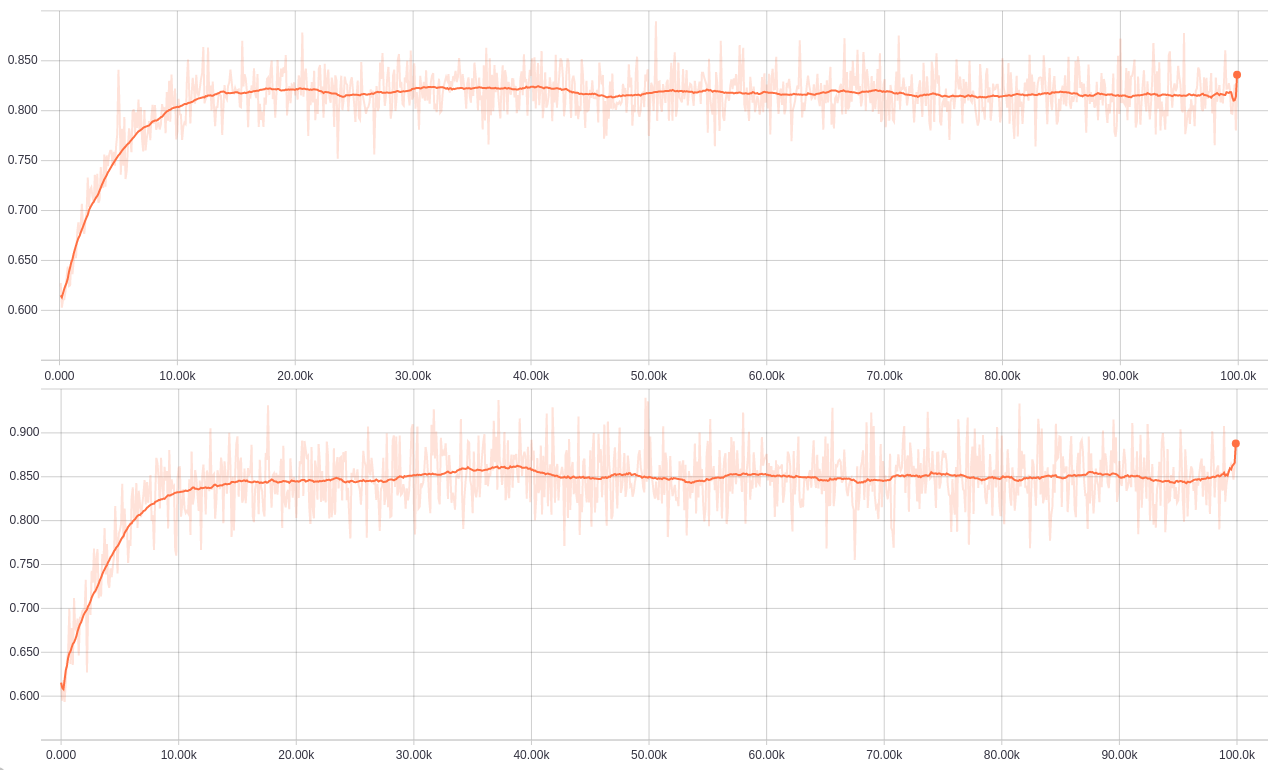
\includegraphics[width=\linewidth]{img/badanie_1.png}
%	\caption{Dokładność na zbiorze walidacyjnym (górny wykres) i uczącym (dolny wykres)}
%	\label{rys:badanie-1}
%\end{figure}
%
%% TODO dodać obrazek przedstawiający graf operacji


\section{Plan badań} \label{sec:plan-badan}
Celem niniejszej pracy magisterskiej jest sprawdzenie jak istotny wpływ na~dokładność klasyfikacji mają 2~czynniki:
\begin{itemize}
    \item regularyzacja typu L2 (\ref{sssec:reg_L2}),
    \item normalizacja lokalnej odpowiedzi (\ref{sssec:normalizacja_odpowiedzi}).
\end{itemize}

W~artykule ,,Practical Recommendations for Gradient-Based Training of Deep Architectures''
(\cite{practical-gradient-based}) skrótowo omówiono problem doboru hiperparametrów sieci. Jednym ze~sposobów
przedstawionych w~opracowaniu jest określenie wartości brzegowych dla~optymalizowanych hiperparametrów,
a~następnie zbadanie przestrzeni między nimi. Po~zbadaniu zachowania sieci dla~tej przestrzeni hiperparametrów, można podjąć
decyzję o~przyjęciu jednego z~zestawów hiperparametrów dla~sieci lub~rozszerzyć pole poszukiwań o~kolejne obszary.

Dla~parametru regularyzacji~L2 (tzw.~\textbf{weight decay}) jako~górne ograniczenie przyjęto początkowo wartość~0.05.
Wybór bazował na~tym, że~w~podobnych sieciach, tj.~przeznaczonych do~identyfikacji obiektów przedstawianych na~obrazkach
z~bazy ImageNet (\cite{imagenet}), wartość tego hiperparametru nie~przekraczała~0.03. Badanie miało sprawdzić
również jak~sieć zachowywałaby~się~bez regularyzacji wag. Stąd jako dolne ograniczenie przyjęto wartość~0.

Dla~parametru decydującego o~wpływie normalizacji lokalnej odpowiedzi (tzw.~parametr $\alpha$) jako ograniczenie górne
przyjęto początkowo wartość~0.001, a~jako ograniczenie dolne wartość~0. Usprawiedliwienie dla~tych decyzji było
takie samo, jak~dla~wyborów dokonanych przy~hiperparametrze regularyzacji~L2.

Dla~każdej pary parametrów sieć była uczona mini-zestawami danych (\textit{ang.~minibatch}), z~których
każdy zawierał 128 przykładów uczących. Po~każdym kroku uczenia pojedynczym mini-zestawem danych, sprawdzano
dokładność sieci na~zbiorze testowym. Po~wykonaniu wszystkich kroków uczenia dla~danej pary hiperparametrów
brano średnią dokładność sieci na~zbiorze testowym ze~100 ostatnich kroków uczenia.

\section{Badanie architektury podstawowej} \label{sec:badanie-1}
W~pierwszym badaniu przeprowadzono proces uczenia sieci o~architekturze opisanej w~sekcji
\ref{ssec:architektura-podstawowa}. Wykorzystano 100 tys. mini-zestawów danych (\textit{ang.~minibatch}).
Wyniki eksperymentu przedstawiono w~tabeli \ref{table:wyniki1}.

\begin{table}[H]
    \centering
    \begin{tabular}{|l|l|l|l|l|l|}
      \hline
                       & $\lambda$ = 0.0005 & $\lambda$ = 0.001 & $\lambda$ = 0.005 & $\lambda$ = 0.01 & $\lambda$ = 0.05 \\
      \hline
      $\alpha=0.00001$ & 0.83 & 0.79 & 0.76 & 0.75 & 0.78 \\
      \hline
      $\alpha=0.00005$ & 0.82 & 0.80 & 0.77 & 0.78 & 0.75 \\
      \hline
      $\alpha=0.0001$  & 0.84 & 0.81 & 0.80 & 0.73 & 0.77 \\
      \hline
      $\alpha=0.0005$  & 0.85 & 0.83 & 0.84 & 0.81 & 0.79 \\
      \hline
      $\alpha=0.001$   & 0.84 & 0.84 & 0.82 & 0.78 & 0.76 \\
      \hline
    \end{tabular}
    \caption{Wpływ regularyzacji L2 ($\lambda$) i~normalizacji lokalnego kontrastu ($\alpha$) na~dokładność klasyfikacji
    sieci neuronowej}
    \label{table:wyniki1}
\end{table}

Całkowity czas badania wyniósł: 40 godzin 10 minut i 58 sekund.

\subsection{Omówienie wyników badań}
Wyniki uzyskane w~badaniu wskazują, że~wraz ze~wzrostem wpływu regularyzacji~L2 na~sieć neuronową, dokładność
klasyfikacji ulegała pogorszeniu. Jednocześnie najlepsze wyniki osiągane były dla~wartości $\alpha$ w~okolicach 0.0005.

W~przypadku wpływu normalizacji lokalnego kontrastu wyniki są~zgodne z~oczekiwaniami, tj.~dla~odpowiednio dobranych
parametrów normalizacja ta~przynosi poprawę rezultatów. Sprzeczne z~przewidywaniami okazały się~zmiany wartości
dokładności dla~różnych wartości parametru $\lambda$. Spodziewano się, że~regularyzacja zapobiegając przeuczeniu
polepszy dokładność klasyfikacji.

Wytłumaczeniem takiego stanu rzeczy może być brak wystąpienia zjawiska przeuczenia, z~dwóch powodów:
\begin{itemize}
    \item zbyt mała liczba neuronów w~sieci, a~przez~to~niska szansa na~zbytnie dopasowanie się~sieci do~danych
          wejściowych,
    \item zbyt mała liczba iteracji podczas uczenia sieci.
\end{itemize}
Regularyzacja~L2 choć~zapobiega wystąpieniu przeuczenia, to~jednak ma~negatywny wpływ na~szybkość uczenia się~sieci,
przez~co~potrzebna jest większa liczba iteracji w~procesie uczenia, aby~osiągnąć zadowalający poziom dokładności.

By~sprawdzić czy~występuje przeuczenie warto posłużyć się~wykresem przedstawiającym dokładność (\textit{ang.~accuracy})
w~zależności od~numeru iteracji uczenia. Na~wykresie \ref{rys:badanie-1} zamieszczono
dokładności liczone na~zbiorze uczącym oraz na~zbiorze walidacyjnym. W~przypadku wystąpienia przeuczenia na~wykresie
powinno się zaobserwować, że~dla~pewnego numeru iteracji pomimo zwiększania się~dokładności na~zbiorze uczącym,
dokładność na~zbiorze walidacyjnym maleje. Na~wykresie \ref{rys:badanie-1} nie~obserwujemy takiej sytuacji.

\begin{figure}[H]
	\centering
	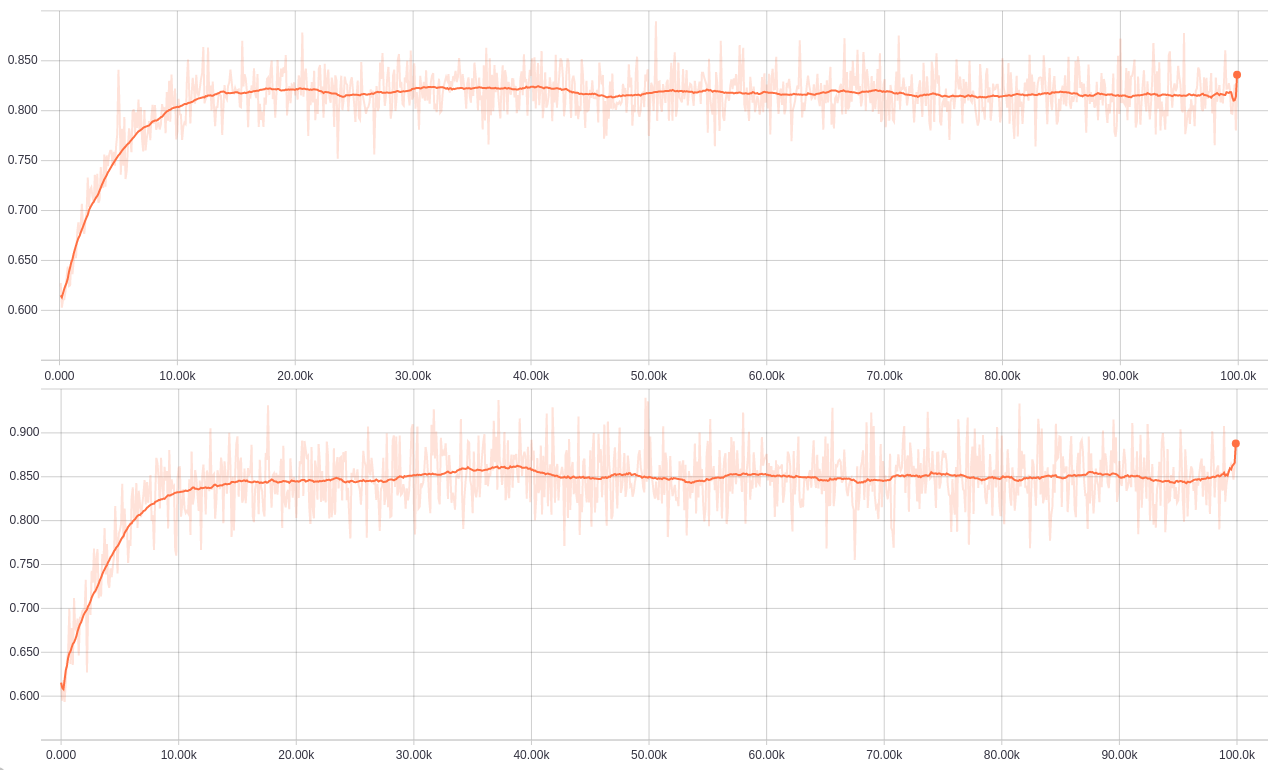
\includegraphics[width=\linewidth]{img/badanie_1.png}
	\caption{Dokładność na zbiorze walidacyjnym (górny wykres) i uczącym (dolny wykres)}
	\label{rys:badanie-1}
\end{figure}

\section{Badanie sieci przy~zwiększonej liczbie iteracji}
W~badaniu nr~2~powtórzono badanie nr~1 (\ref{sec:badanie-1}) ze~zwiększoną liczbą iteracji (do 144000).
Spodziewano się,~że~od~pewnego numeru iteracji będzie obserwowany spadek dokładności na~zbiorze walidacyjnym
przy~jednoczesnym wzroście dokładności na~zbiorze uczącym. Jednakże również nie~udało się~zaobserwować zaistniałej
sytuacji (patrz wykres~\ref{rys:badanie-2}). Prawdopodobnie wynika to~z~tego, że~sieć z~powodu swojej względnie prostej
struktury nie~ma~możliwości przeuczenia się~(zbyt mała liczba neuronów w~stosunku do~liczby przykładów uczących).

\begin{figure}[H]
	\centering
	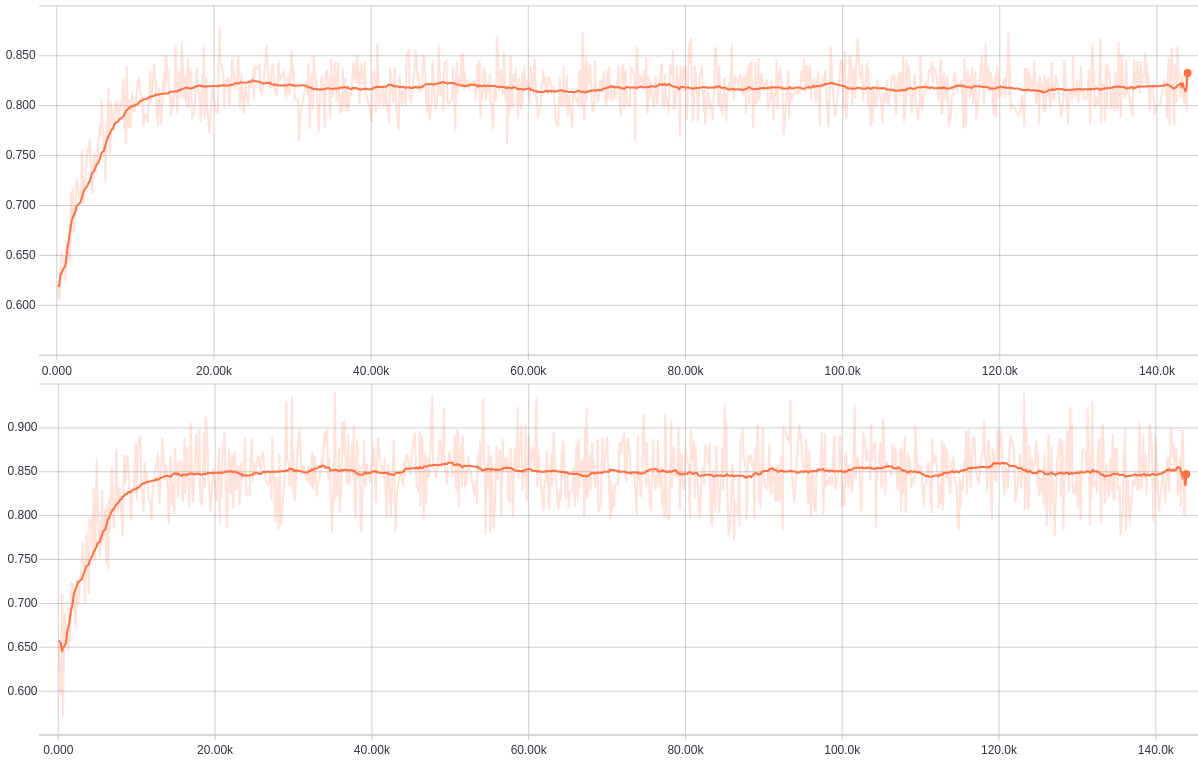
\includegraphics[width=\linewidth]{img/badanie_2.png}
	\caption{Dokładność na zbiorze walidacyjnym (górny wykres) i uczącym (dolny wykres) przy~liczbie iteracji
	         zwiększonej do~144 tysięcy}
	\label{rys:badanie-2}
\end{figure}

Wyniki przedstawiono w~tabeli \ref{table:wyniki2}.

\begin{table}[H]
    \centering
    \begin{tabular}{|l|l|l|l|l|l|}
      \hline
                       & $\lambda$ = 0.0005 & $\lambda$ = 0.001 & $\lambda$ = 0.005 & $\lambda$ = 0.01 & $\lambda$ = 0.05 \\
      \hline
      $\alpha=0.00001$ & 0.90 & 0.89 & 0.87 & 0.83 & 0.82 \\
      \hline
      $\alpha=0.00005$ & 0.91 & 0.88 & 0.85 & 0.83 & 0.84 \\
      \hline
      $\alpha=0.0001$  & 0.90 & 0.88 & 0.88 & 0.87 & 0.87 \\
      \hline
      $\alpha=0.0005$  & 0.92 & 0.92 & 0.89 & 0.87 & 0.86 \\
      \hline
      $\alpha=0.001$   & 0.89 & 0.87 & 0.87 & 0.83 & 0.83 \\
      \hline
    \end{tabular}
    \caption{Wpływ regularyzacji L2 ($\lambda$) i~normalizacji lokalnego kontrastu ($\alpha$) na~dokładność klasyfikacji
    sieci neuronowej przy~liczbie iteracji zwiększonej do~144 tysięcy}
    \label{table:wyniki2}
\end{table}

Całkowity czas badania wyniósł: 64 godziny 17 minut i 23 sekundy.


\section{Badanie na zmniejszonym zbiorze uczącym}
By~sprawdzić jaki wpływ na~dokładność klasyfikacji będzie miała regularyzacja, gdy~problem przeuczenia występuje,
zaprojektowano badanie numer~3, w~którym sześciokrotnie zmniejszono liczbę przykładów w~zbiorze uczącym (przy~zachowaniu
takiego samego rozmiaru zbioru walidacyjnego). Spodziewano się,~że~spowoduje to~wystąpienie zjawiska przeuczenia sieci
(\textit{ang.~overfitting}).

\begin{figure}[H]
	\centering
	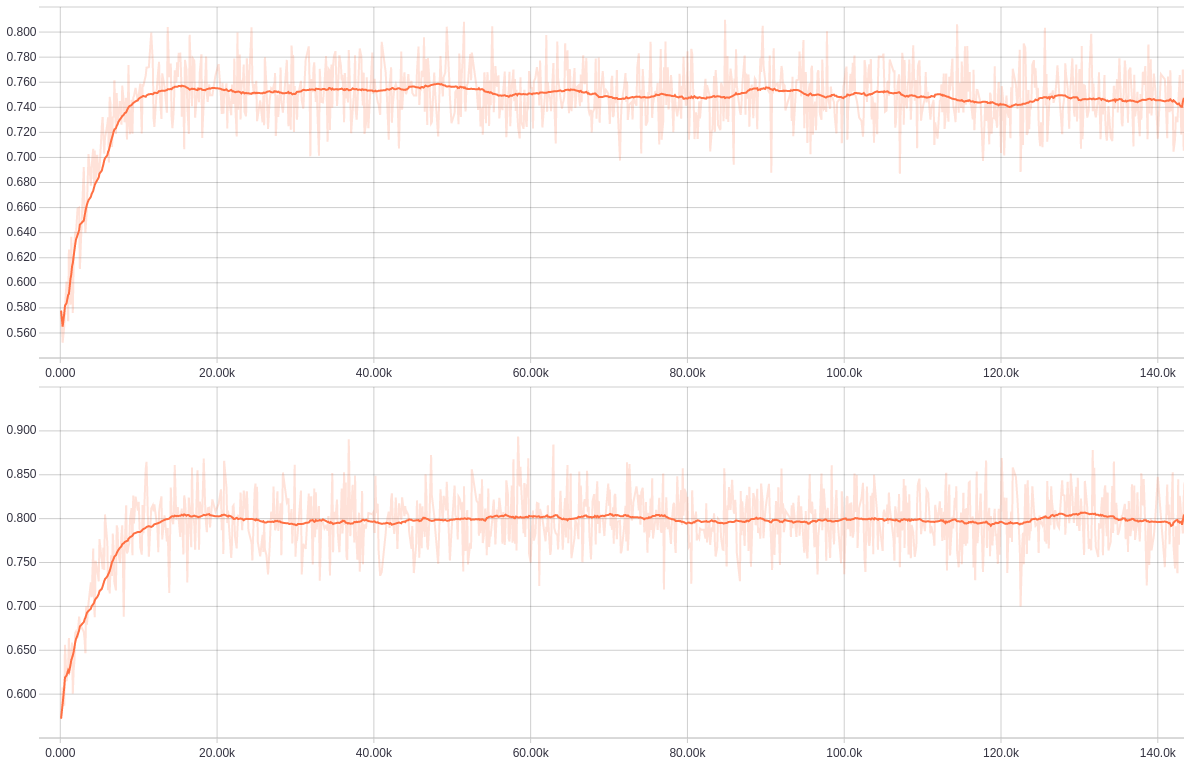
\includegraphics[width=\linewidth]{img/badanie_3.png}
	\caption{Dokładność na zbiorze walidacyjnym (górny wykres) i uczącym (dolny wykres) przy~sześciokrotnie
	         zmniejszonym zbiorze uczącym. Liczba iteracji: 144 tysiące}
	\label{rys:badanie-3}
\end{figure}

Jak~widać na~wykresie \ref{rys:badanie-3} problem przeuczenia zaczyna się~pojawiać w~okolicach iteracji nr~45000.
Stąd należy się~spodziewać, że~regularyzacja zmniejszy występowanie tego niepożądanego zjawiska.

W~tabeli \ref{table:wyniki3} przedstawiono dokładność klasyfikacji dla~różnych kombinacji parametrów normalizacji
i~regularyzacji. Tak~jak~się~spodziewano regularyzacja przy~odpowiednio dobranych metaparametrach
($\alpha=0.0005$ i~$\lambda=0.001$) poprawia jakość klasyfikacji.

\begin{table}[H]
    \centering
    \begin{tabular}{|l|l|l|l|l|l|}
      \hline
                       & $\lambda$ = 0.0005 & $\lambda$ = 0.001 & $\lambda$ = 0.005 & $\lambda$ = 0.01 & $\lambda$ = 0.05 \\
      \hline
      $\alpha=0.00001$ & 0.76 & 0.80 & 0.74 & 0.69 & 0.69 \\
      \hline
      $\alpha=0.00005$ & 0.78 & 0.77 & 0.72 & 0.69 & 0.67 \\
      \hline
      $\alpha=0.0001$  & 0.77 & 0.78 & 0.79 & 0.74 & 0.73 \\
      \hline
      $\alpha=0.0005$  & 0.78 & 0.82 & 0.76 & 0.76 & 0.72 \\
      \hline
      $\alpha=0.001$   & 0.76 & 0.79 & 0.76 & 0.69 & 0.69 \\
      \hline
    \end{tabular}

    \caption{Wpływ regularyzacji L2 ($\lambda$) i~normalizacji lokalnego kontrastu ($\alpha$) na~dokładność klasyfikacji
    sieci neuronowej przy~sześciokrotnie zmniejszonym zbiorze uczącym. Liczba iteracji: 144 tysiące}
    \label{table:wyniki3}
\end{table}

Całkowity czas badania wyniósł: 62 godziny 43 minuty i 27 sekund.

\section{Weryfikacja poprawności działania sieci} \label{sec:weryfikacja-poprawnosci}
Po~dobraniu hiperparametórw sieci warto wykonać badanie pomocnicze mające na celu sprawdzić czy~przy~klasyfikacji
obrazów są~brane pod~uwagę właściwe piksele np.~czy~przy~klasyfikacji obrazu na~którym jest pies, sieć stwierdza,
że~jest to~pies na~podstawie fragmentu obrazu przedstawiającego psa czy~na~podstawie fragmentów nieistotnych.

Przy~poszukiwaniu odpowiedzi na~pytanie: "co~sieć bierze pod~uwagę przy~klasyfikacji obrazów" warto wykorzystać
metody przedstawione w~artykule ,,Visualizing and Understanding Convolutional Networks'' (\cite{understanding-cnn}).
Jedną z~nich~jest metoda, w~której zasłaniane są różne fragmenty klasyfikowanego obrazu i~sprawdzane jest,
jaki ma~to~wpływ na~klasyfikację, a~dokładniej: na~wartość prawdopodobieństwa, że~na~danym obrazku znajduje
się~określony przedmiot.

Przesuwając odpowiednio łatkę (czyli fragment obrazu, który jest ,,zasłaniany'' poprzez zastąpienie go zerami),
uzyskujemy kolejne wartości prawdopodobieństwa, że~na~obrazie znajduje się~przedmiot, który naprawdę się~na~nim
znajduje. Następnie w~utworzonej mapie ciepła na~pozycjach pikseli istotnych z~punktu widzenia klasyfikacji wystąpią
niskie wartości prawdopodobieństwa (co~oznacza, że~po~zasłonięciu tego fragmentu, prawdopodobieństwo poprawnej
klasyfikacji będzie niskie). Natomiast punkty o~wysokiej wartości prawdopodobieństwa odpowiadać będą pikselom
nieistotnym.

\begin{figure}[H]
	\centering
	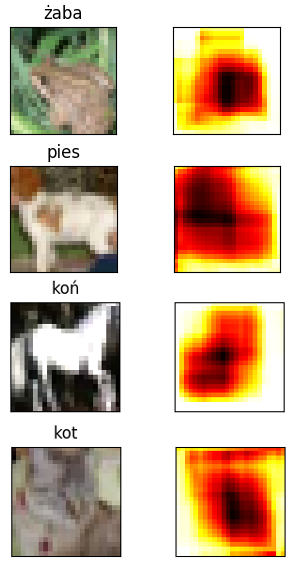
\includegraphics[width=0.75\linewidth]{img/heatmap.png}
	\caption{Mapy ciepła ilustrujące, jak istotne dla klasyfikacji są dane piksele. Im~piksel ciemniejszy, tym~jest
	ważniejszy. W~pierwszej kolumnie znajdują się~klasyfikowane obrazki, a~w~drugiej odpowiadające im~mapy ciepła}
	\label{rys:badanie-3}
\end{figure}

\section{Wnioski końcowe}
Jak~pokazały przeprowadzone badania zabiegi takie jak~regularyzacja nie~zawsze mają sens. Należy je~stosować wyłącznie
wtedy, kiedy obserwowane jest przeuczenie sieci. W~przeciwnym wypadku zamiast zwiększania jakości klasyfikacji
(wyrażanego jako dokładność), obserwowany jest jej~spadek.

By~sprawdzić czy~przeuczenie sieci występuje warto posłużyć się~wykresem przedstawiającym dokładność sieci na~zbiorze
uczącym i~walidacyjnym mierzoną po~każdej iteracji uczenia. Innym badaniem, które pozwala sprawdzić czy~sieć bierze
pod~uwagę istotne informacje na~zdjęciu jest wykorzystanie map ciepła, w~których im~piksel miał większy wpływ
na~wynik klasyfikacji, tym~,,cieplejszy'' ma kolor (patrz sekcja \ref{sec:weryfikacja-poprawnosci}).

Odpowiednie dobranie metaparametrów sieci nie~jest łatwe. Zwykle dobrze jest bazować na~architekturze innej sieci
wykonującej podobne zadanie (przy~zbiorze \mbox{CIFAR-10} może to~być np.~sieć AlexNet). Następnie w~celu poprawy jakości
klasyfikacji można wykorzystać przeszukiwanie kratowe (\textit{ang.~grid search}), które opisano
w~sekcji~\ref{sec:plan-badan}.
